\documentclass{standalone}
\usepackage{tikz}
\usetikzlibrary{math}
\usetikzlibrary{decorations.pathreplacing}
\usetikzlibrary{decorations.markings}
\usetikzlibrary{calc}
\usetikzlibrary{arrows.meta}

\usepackage{pgfplots}
\pgfplotsset{compat=1.8}



\begin{document}

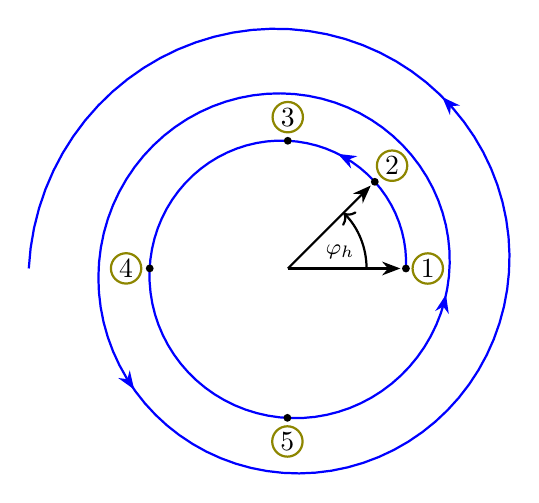
\begin{tikzpicture}
\pgfmathsetmacro{\alpha}{0.05}
\pgfmathdeclarefunction{spirale}{1}{\pgfmathparse{1.5*exp(\alpha*#1)}}

\draw[domain=0:5*pi,samples=200, blue, thick]
plot ({deg(\x)}:{spirale(\x)})
[postaction={
    decorate,
    decoration={
        markings,
        mark=between positions 0.05 and 1 step 0.25 with {\arrow{Stealth}},
}},
postaction={
    decorate,
    decoration={
        markings,
        mark=at position 0.0 with {\node[circle, fill=black, inner sep=1] {}; \node[circle, black, right, xshift={2pt},
        draw=olive, inner sep=1pt] {1};},
        mark=at position 0.0335 with {\node[circle, fill=black, inner sep=1] {}; \node[circle, black,
        shift={(43:0.3cm)}, draw=olive, inner sep=1pt] {2};},
        mark=at position 0.0685 with {\node[circle, fill=black, inner sep=1] {}; \node[circle, black,
        shift={(90:0.3cm)}, draw=olive, inner sep=1pt] {3};},
        mark=at position 0.1425 with {\node[circle, fill=black, inner sep=1] {}; \node[circle, black,
        shift={(180:0.3cm)}, draw=olive, inner sep=1pt] {4};},
        mark=at position 0.2225 with {\node[circle, fill=black, inner sep=1] {}; \node[circle, black,
        shift={(270:0.3cm)}, draw=olive, inner sep=1pt] {5};},
    }
}];

\draw[-Stealth, thick, shorten >=2pt] (0,0) -- +(0:{spirale(0)});
\draw[-Stealth, thick, shorten >=2pt] (0,0) -- +(45:{spirale(rad(45))});
\draw[thick, ->] (0:1) arc[start angle=0, end angle=45, radius=1];
\node at (18:0.7) {\footnotesize $\varphi_{h}$};

\end{tikzpicture}

\end{document}